\chapter{Results: Imaging}
\label{imaging}

\emph{\color{red}do corr. on p-meter sensitive A ($\times$1.57) and 89 percent optical flat T}

Results presented in Chapter 4 determined the ideal conditions for imaging small numbers of Ba atoms in SXe.  Ideal excitation wavelengths were determined by studying the excitation spectra of the signal as well as the background.  Bleaching of the fluorescence determined ideal laser intensities to be used.  Studies of deposits made and observed at different temperatures determined the procedure of depositing at $50 \pm 5$~K and observing at 11~K.  Imaging of the 577- and 591-nm fluorescence is presented in \ref{sec:imaging590and577} down to the $10^{4}$-atom level, and imaging of the 619-nm peak is presented down to the single-atom level.  Initial scanned images of Ba\textsuperscript{+} deposits are presented in \ref{sec:scanning}.

Though the imaging spectrometer can produce spacial images with the 0-order grating reflection, better collection efficiency and imaging quality are achieved by removing the spectrometer and imaging directly onto the CCD.  Band-pass filters were used to pass the desired Ba fluorescence peak(s) while attenuating laser scatter and sapphire fluorescence.

%angle=90,
\begin{figure} %[H]
        \centering
                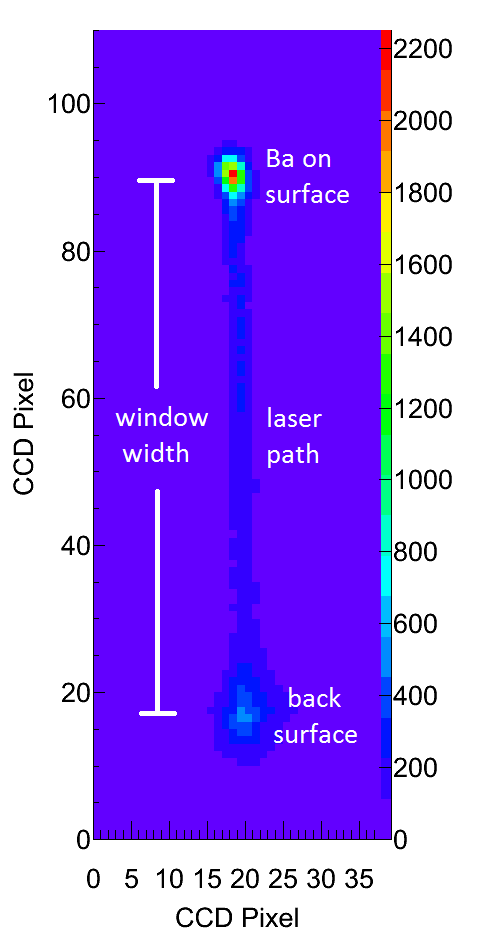
\includegraphics[width=.4\textwidth]{figures/raw_14-atom_labels_from_paper_1f.png}
                \caption{Example image of focused laser spot on a Ba\textsuperscript{+} deposit on a c-plane sapphire window of 0.5~mm thickness surface.  A 620-nm band-pass filter passes the fluorescence.}
\label{fig:imageexamp}
\end{figure}

An example image of the focused 570~nm dye laser on a Ba\textsuperscript{+} deposit is shown in Fig. \ref{fig:imageexamp}.  With 4$\times$ magnification, each pixel is 5~$\mu$m$\times$5~$\mu$m.  The laser's path through the window is faintly visible by the tail of the broad Cr\textsuperscript{3+} fluorescence in the 620-nm band-pass.  The laser is focused at the top surface of the window, which faces the ion beam.  The surface background is seen on both surfaces.  The observed size of the laser spot, with a 1/e$^{2}$ radius of about 12~$\mu$m, is larger than the 2.06~$\mu$m $\times$ 2.66~$\mu$m 1/e$^{2}$ laser spot size.  Aberrations and vibrations in the collection optics could contribute to this.
% inability to reach the diffraction limit in imaging.

%\begin{wrapfigure}{r}{0.5\textwidth}
  %\begin{center}
   % 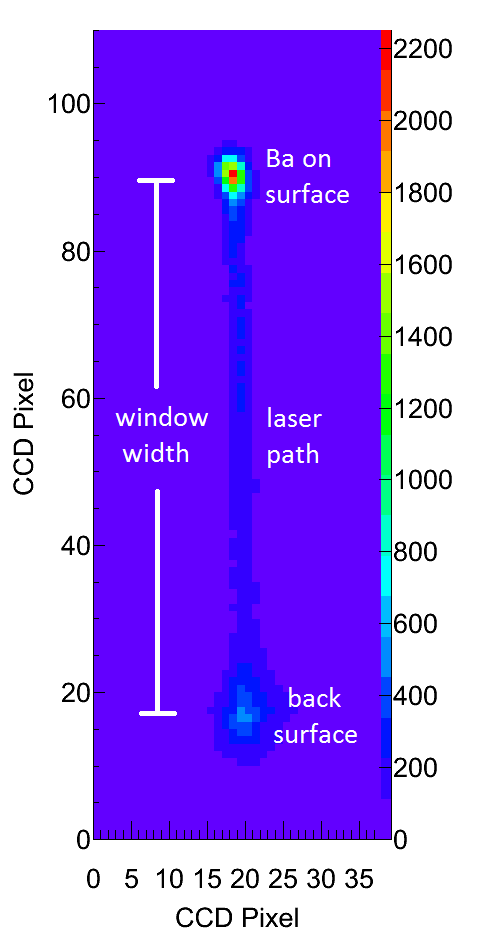
\includegraphics[width=0.35\textwidth]{figures/raw_14-atom_labels_from_paper_1f.png}
  %\end{center}
  %\caption{}
  %\label{fig:imageexamp}
%\end{wrapfigure}

\section{Imaging 577- and 591-nm peaks}
\label{sec:imaging590and577}

\begin{figure} %[H]
        \centering
                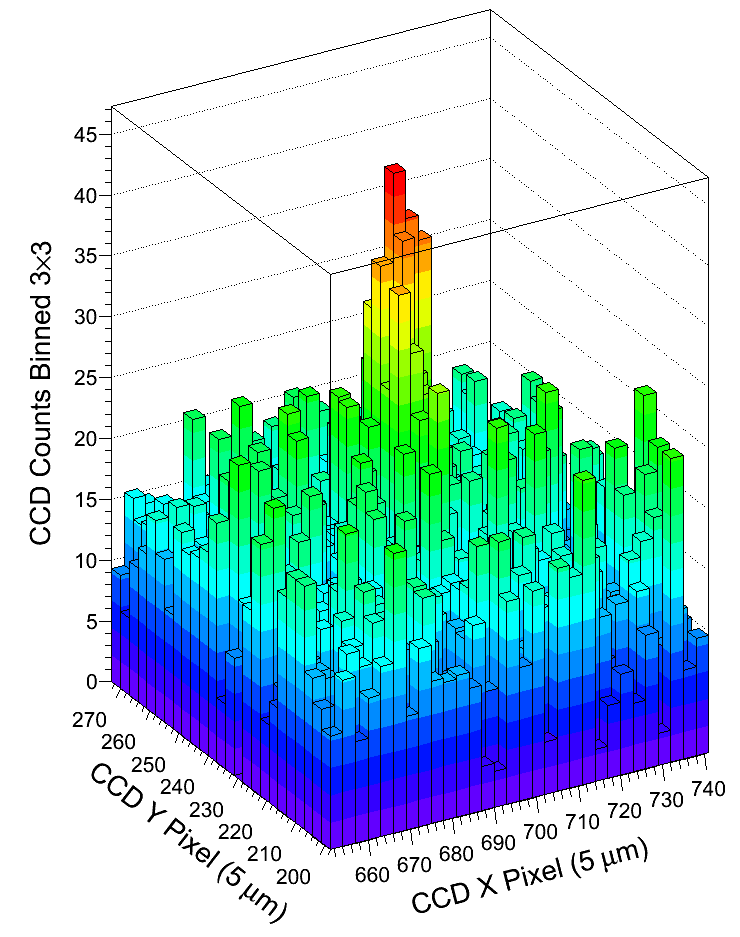
\includegraphics[width=.6\textwidth]{figures/image_1e4.png}
                \caption{Image of about ? average Ba atoms in SXe.  100-s exposure with .02~$\mu$W of 566~nm excitation, deposited at 50~K and observed at 11~K.  $3 \times 3$ CCD pixel binning.}
\label{fig:image590s}
\end{figure}

First attempts at imaging small numbers of Ba atoms in a focused laser region were done with the 577- and 591-nm Ba fluorescence peaks together using a 586-nm band-pass filter, which passes 573 - 599~nm FWHM.  This filter has a 2" diameter, resulting in a factor of 4$\times$ more collection efficiency.  An image of x atoms on average, with x total atoms exposed, is shown in Fig. \ref{fig:image590s} for a 100-s exposure with 0.02~$\mu$W of 566-nm excitation.  The distinction between average and total is described in Sec. \ref{sec:vibes}.  At this low intensity, no bleaching was observed in the four frames observed (frame 1 is shown).  Groups of 9 ($3 \times 3$) CCD pixels are binned to produce the nice peak shown.  As discussed in \ref{sec:bleaching}, detection of very small numbers of atoms in these sites may require several re-pump lasers.  As a result of low total exposure, neither the sapphire nor the surface backgrounds are present in these images, though a Xe-only image has been subtracted. 

%$5 \times 10^{3}$        $\leq$ 10$^{4}$

%(10$^{4}$ Ba\textsuperscript{+} ions deposited into the effective laser region)

%Bleaching data was used to optimize laser intensity and exposure time to achieve maximal signal in frame 1, and to avoid hole bleaching.  The fast bleaching of these peaks is the limiting factor on sensitivity.

\section{Imaging 619-nm peak}
\label{sec:imaging619}

\begin{figure} %[H]
        \centering
                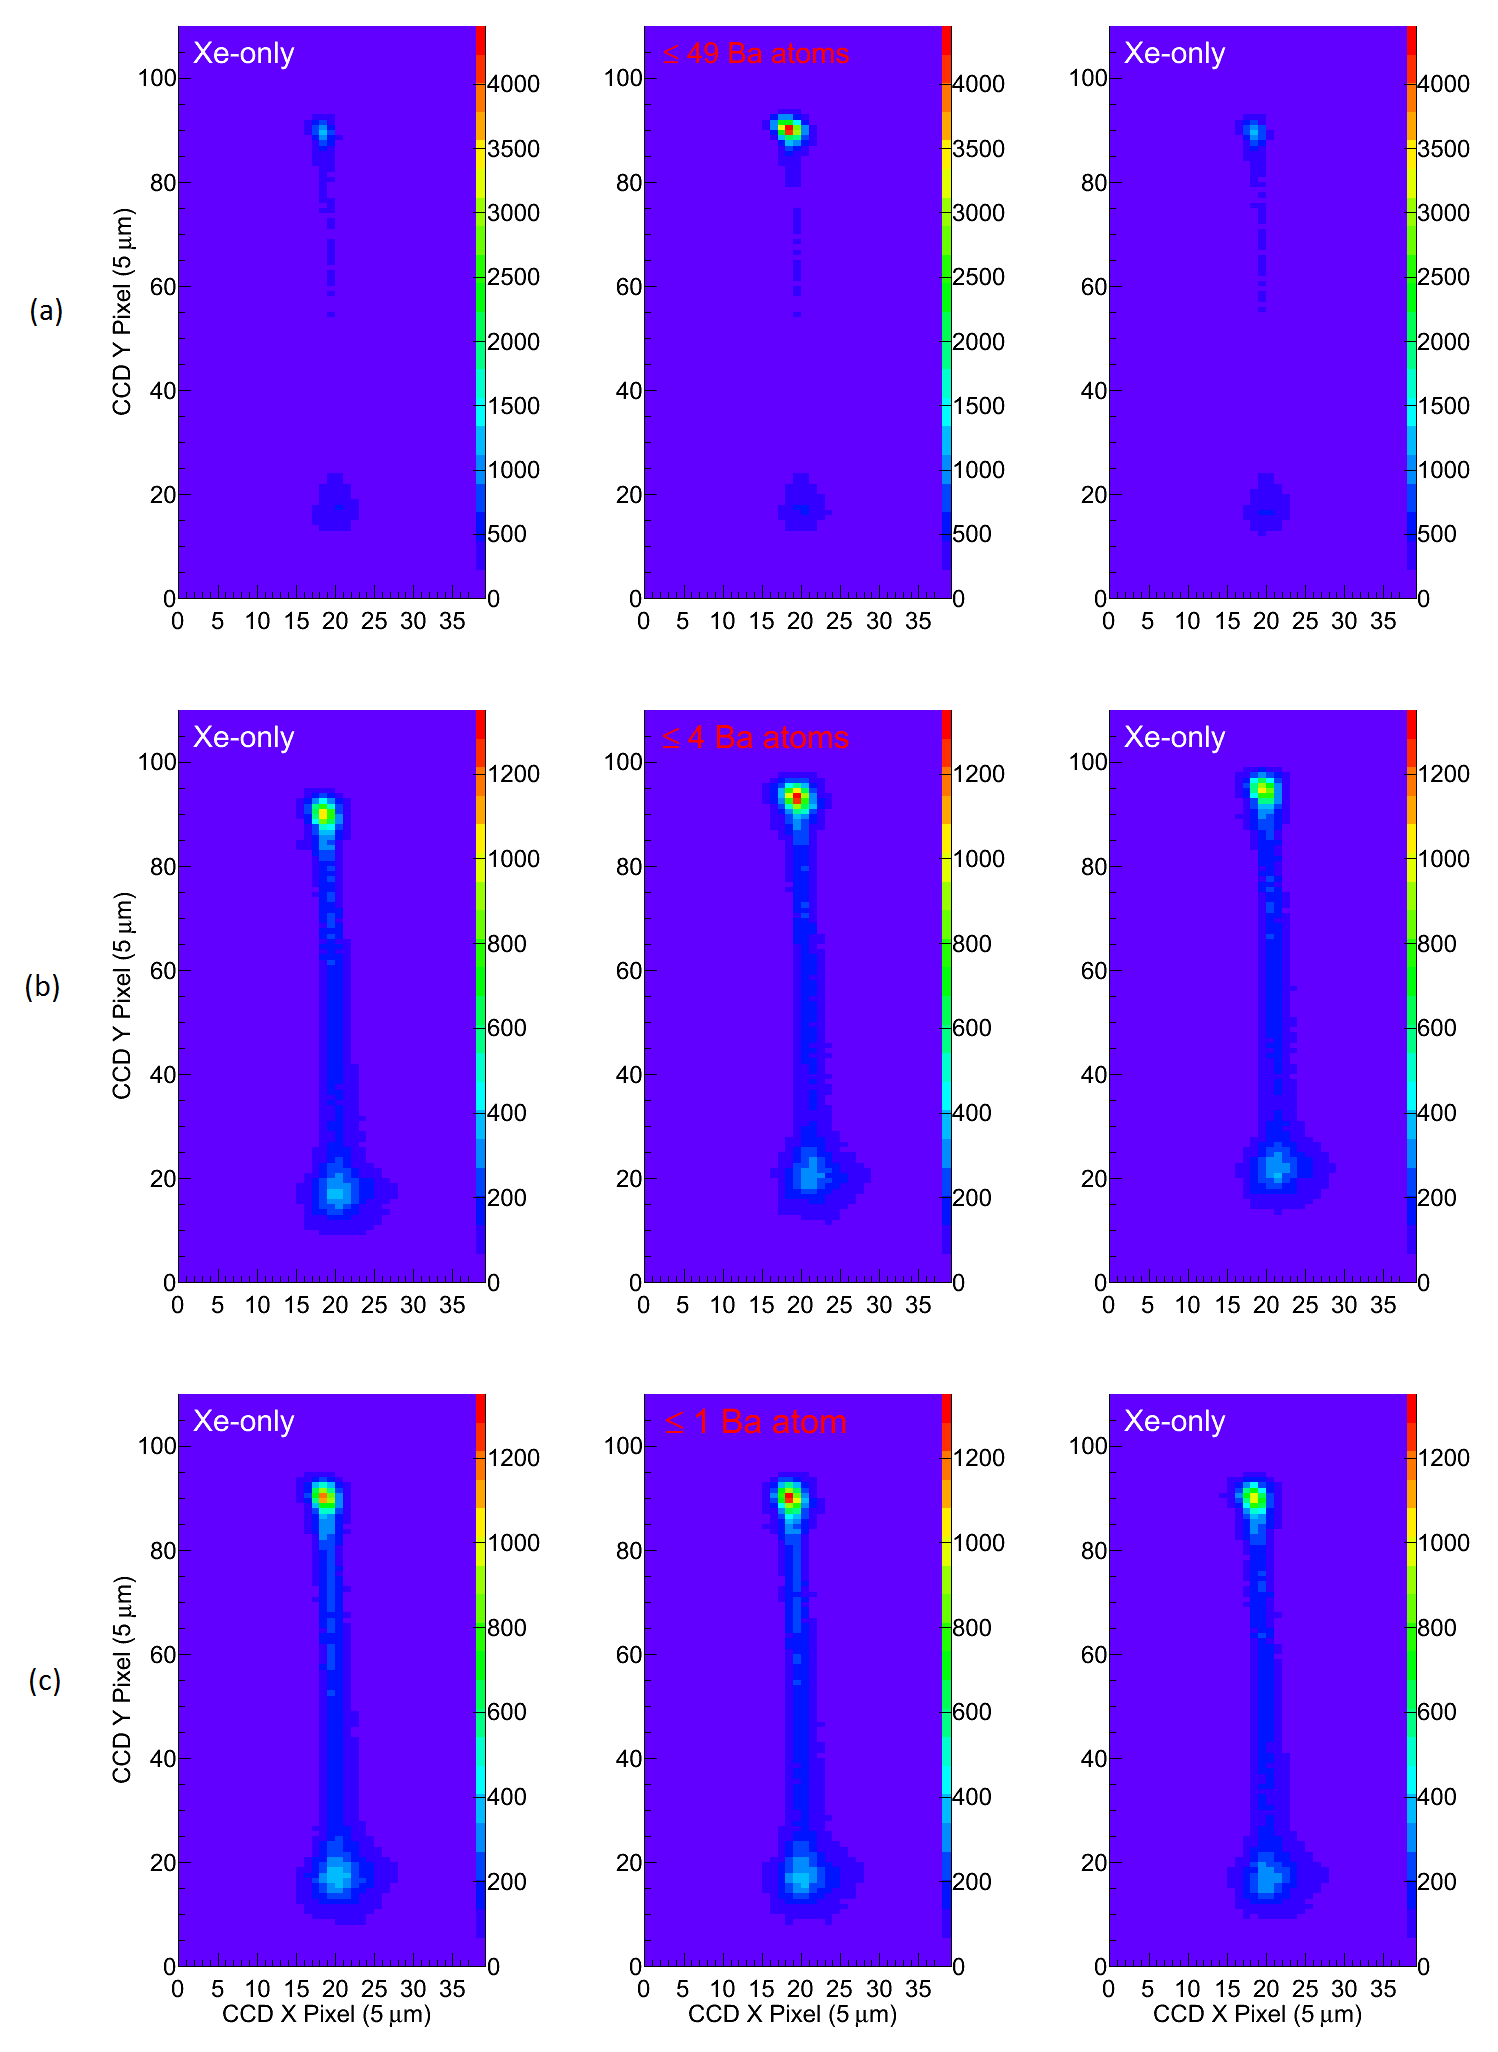
\includegraphics[width=.95\textwidth]{figures/xebaxe_average.png}
                \caption{Raw images of three Ba\textsuperscript{+} deposits yielding (a) $\leq 49$, (b) $\leq 4$, and (c) $\leq 1$ average Ba atoms, with their preceding and succeeding Xe-only deposits.}
\label{fig:xebaxe}
\end{figure}

%This paragraph is kind of dumb and maybe not even necessary:
%At low laser intensities, the 619-nm peak appears minor compared to the 577- and 591-nm peaks.  However, its much lower bleaching rate brings it to dominate over larger exposures, e.g. with the intensity of a focused laser at 0.01-0.1~mW over seconds or minutes.  Experiments imaging small numbers of Ba atoms in SXe in a focused laser region with the 619-nm peak were successful down to the single-atom level.

%\begin{figure} %[H]
%        \centering
%                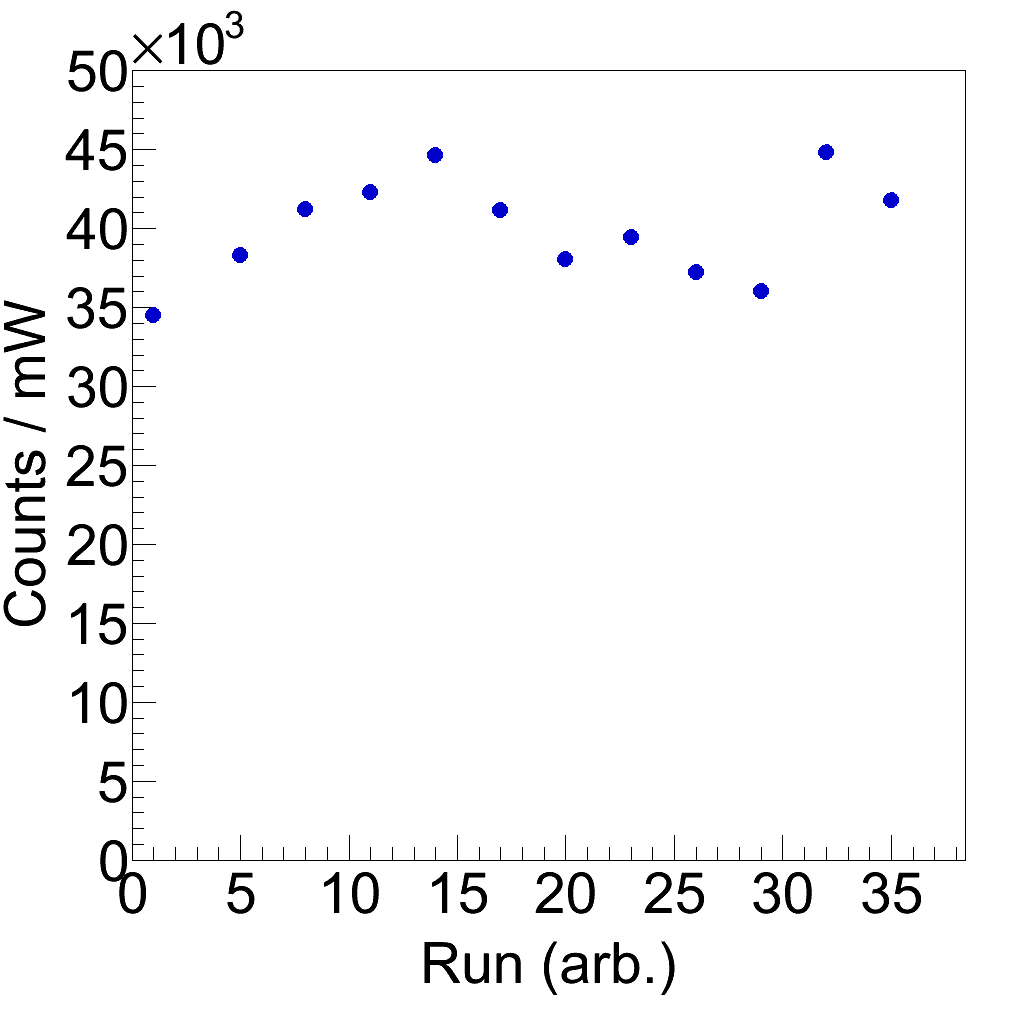
\includegraphics[width=.4\textwidth]{figures/xe_variation.png}
%                \caption{Background counts in focused laser region over the course of an experiment.}
%\label{fig:xevar}
%\end{figure}

Raw images of Ba\textsuperscript{+} deposits and their preceding and succeeding Xe-only deposits are shown in Fig. \ref{fig:xebaxe} for deposits of (a) $\leq 49$ ($\leq 230$), (b) $\leq 4$ ($\leq 20$), and (c) $\leq 1$ ($\leq 5$) average (total) Ba atoms.   Signal is distinguishable from background by eye, even at the 1-atom average signal level.  The lack of historical buildup of Ba fluorescence between deposits, even for large Ba\textsuperscript{+} deposits, is important for the implementation of this method of Ba tagging on a probe in nEXO.

An imaging experiment consisted of many different pulsed Ba\textsuperscript{+} deposits, each of which was evaporated after observation.  This procedure is described in \ref{sec:deposition}-\ref{sec:collection}.  A linear relationship between observed signal and ions deposited must be observed and repeated.  Frequent Xe-only deposits ware made, typically every three runs, to establish the local background.  The image of each deposit was analyzed by summing the counts of a 3-pixel$\times$3-pixel (15$\mu$m$\times$15$\mu$m) region centered on the laser spot in the SXe layer where it excites Ba atoms, i.e. at the top of the laser path in Fig. \ref{fig:imageexamp}.  A partial-bin integrator was implemented such that the 3-pixel$\times$3-pixel region could be centered on the peak center of each run, which typically varied by about half a micron between runs.  Summed counts vs. Ba\textsuperscript{+} ions deposited into the laser region is shown in Fig. \ref{fig:lin} for a combination of data sets from two separate days \emph{\color{blue}maybe you want them separate (with each point having errors) by color to show agreement }  Each point has subtracted the averaged counts from the two surrounding Xe-only deposits.  Some variation in signal is observed, likely due to spatial drifting of the ion beam, as this variation was larger on days where larger beam drift was observed.  Nonetheless, a clear linearity in observed in signal vs. ions deposited, all the way down to single ions deposited.  Recall that the number of ions is an upper limit on the number of atoms in the 619-nm peak matrix site.  ``0-pulse" deposits are also made, wherein Faraday cup 3 is retracted for the 1-s period, but the ion beam remains deflected with no pulses.  This establishes the level of neutral Ba atoms making their way down the beam line from the source into the laser region.  Signal at the few-atom level is observed from these deposits.

Images of Ba fluorescence are produced by subtracting Xe-only images, shown in Fig. \ref{fig:train} .... um were also directly subtracted to produce images of 619-nm Ba fluorescence.  In cases where the image has shifted slightly between runs, a binning redistribution was applied to do sub-pixel image shifting for better subtraction, though images which did not require this were preferred.  619-nm fluorescence images for several deposits of varying numbers of atoms are shown in Fig. \ref{fig:train}.

%... and try combining those other days.  It will require scaling for intensity difference (spher. abb.) and time, and remember different I$\times$t might give different efficiency.

\begin{figure} %[H]
        \centering
                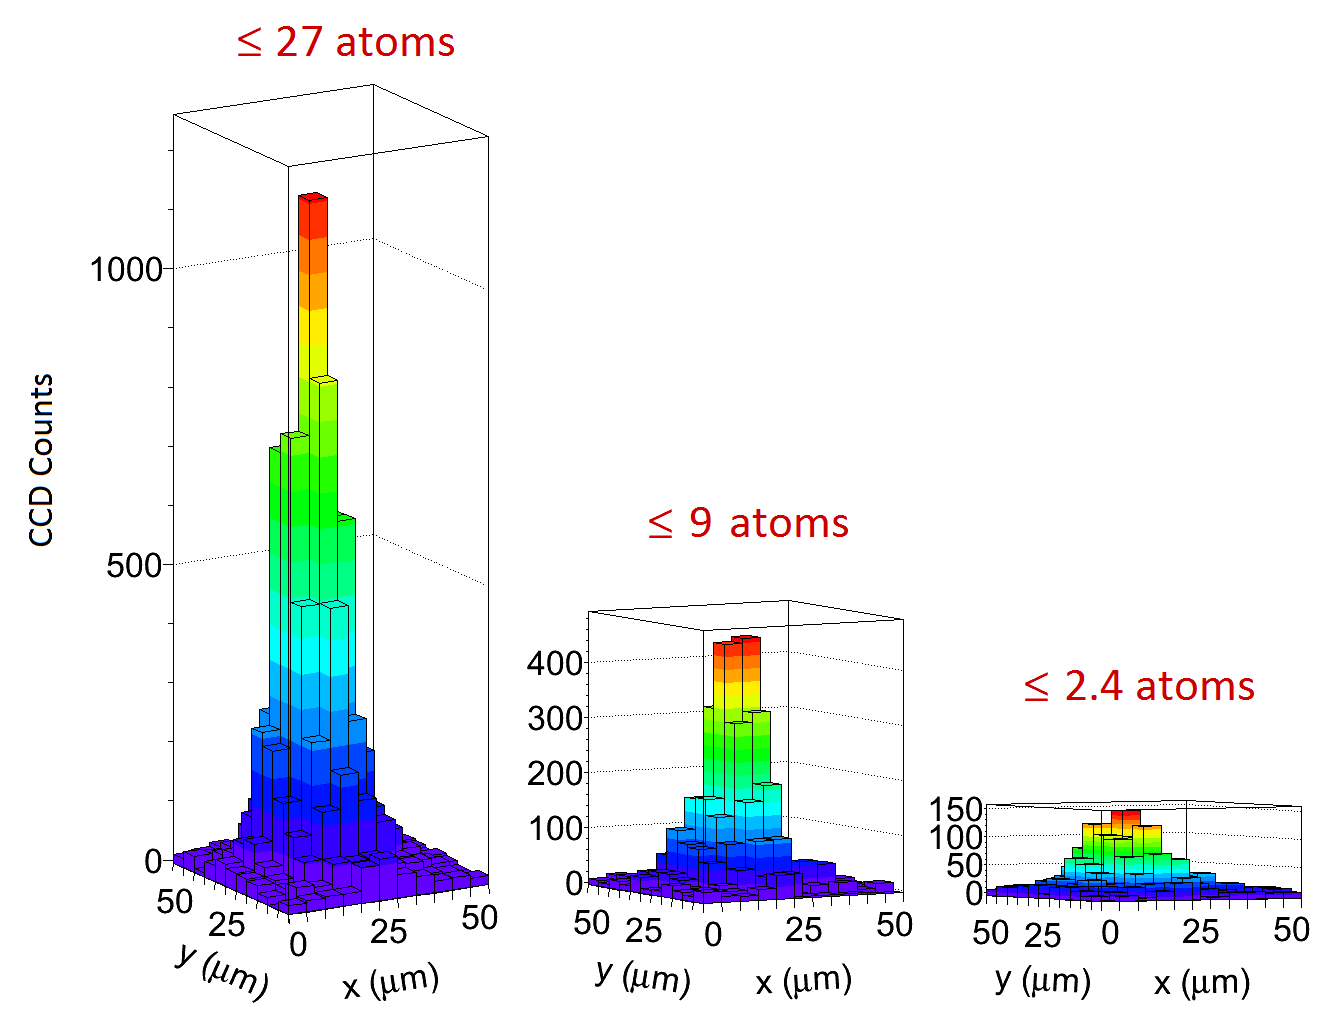
\includegraphics[width=.99\textwidth]{figures/train_20150807_v3_runs70_88_81_fromGiorgioFolder.png}
                \caption{\color{red}will change:  1) have more than this, 2) do pixel (5micron) on axis like others, 3) have same-looking phi angle on all}
\label{fig:train}
\end{figure}

%\emph{\color{gray}Paragraph on BG variation was here, but I moved it to Method w/o thinking thru completely in this context.  Image is also commented out here, above train figure... and actually I took it out there too...}

%Variation in the background level, dominated by the surface background, is shown in Fig. \ref{fig:xevar}.  Variation was most likely caused by drift of the laser position on the window, to regions of different historical bleaching.  Local variations are at the single-atom signal level, however positive signal after subtraction, even at the single-atom level, demonstrates that this variation is sufficiently low.

\begin{figure} %[H]
        \centering
                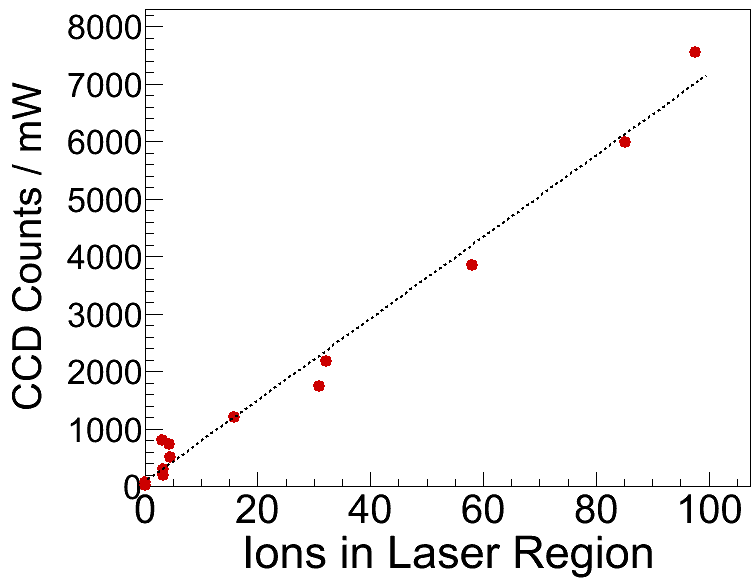
\includegraphics[width=.5\textwidth]{figures/lin_20150526.png}
                ~
                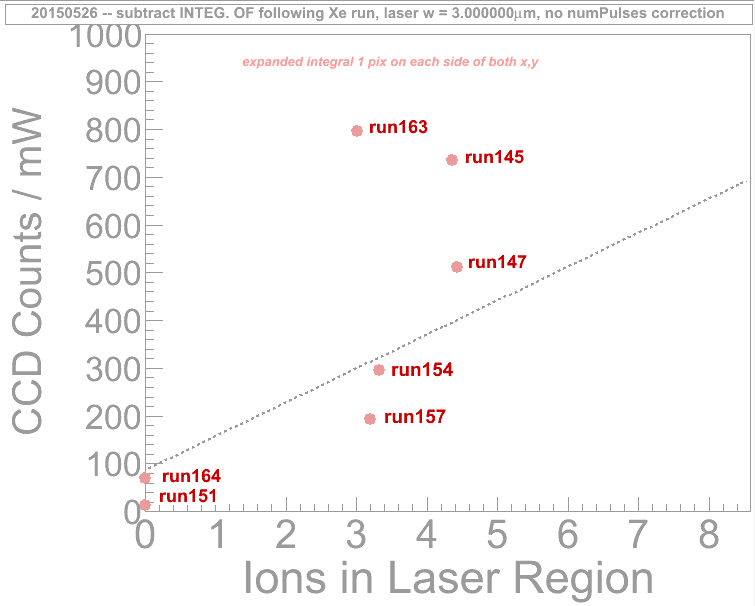
\includegraphics[width=.5\textwidth]{figures/lin_pres_zoom_predictSingleAtom.png}
                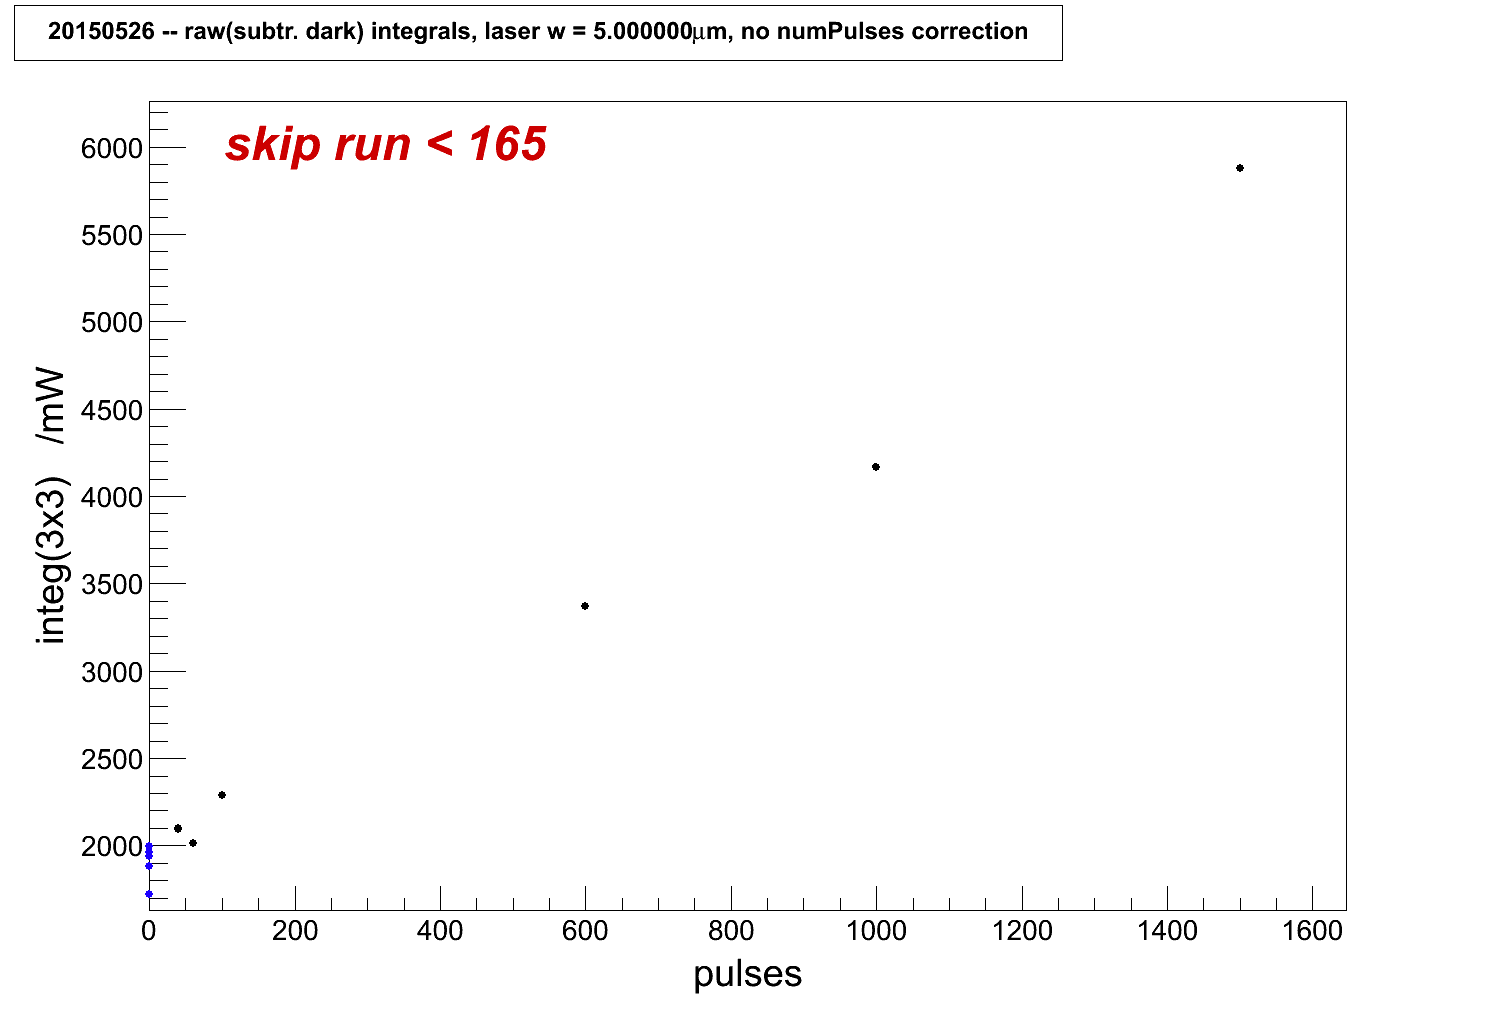
\includegraphics[width=.5\textwidth]{figures/lin_vsPulses_all_3x3_pre-165.png}
                ~
                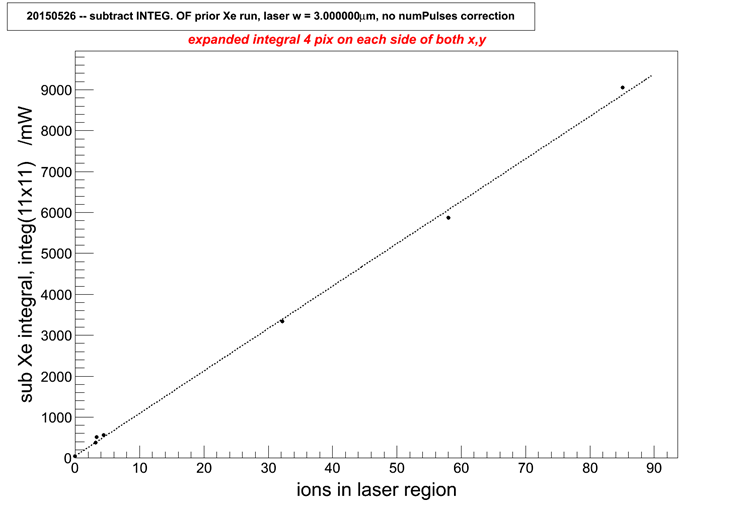
\includegraphics[width=.5\textwidth]{figures/lin_20150526_cut.png}
                \caption{\color{gray}this day looks so good that i think you should use it in some way, w/ area corr of course, maybe and ideally combined with lower number stuff -- maybe the variation in e.g. 8-7 is at same level as that in this data? maybe the lin from this will look boss.  remember it has bi-convex.  Showing w/ Xes, as in 3rd thing, is prolly cool too.}
\label{fig:lintemp}
\end{figure}

\begin{figure} %[H]
        \centering
                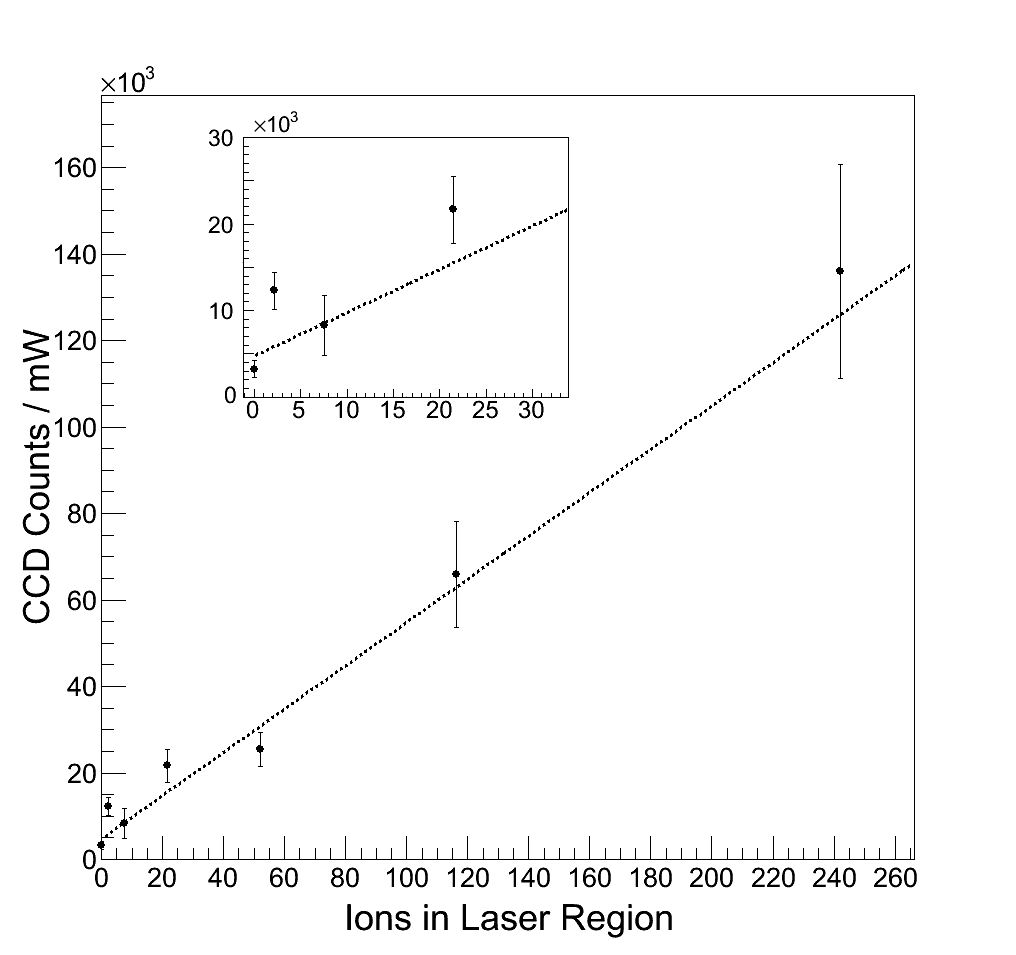
\includegraphics[width=.99\textwidth]{figures/lin_corr_20151016.png}
                \caption{\emph{\color{gray}Probably you would show this after showing actual data and where you are grouping points.}  619-nm signal vs. Ba\textsuperscript{+} deposited in effective excitation region of 17.8~$\mu$m using focused laser at 570~nm. \emph{\color{gray}move y-ax title over, Remove x errors}}
\label{fig:lin}
\end{figure}

\section{Scanned Images}
\label{sec:scanning}

The ultimate demonstration of single-atom imaging would be to scan the focused laser over a sample of separated Ba atoms, observing a peak when the laser moves over each atom.  Preliminary scans were performed by scanning the focusing lens in a grid patter, using the setup described in \ref{sec:laserscanning}.   \emph{\color{gray}choose what to show and what to say about it -- there are some decent things to show really}  [issues are BG, reproduceability, vibrations]

\emph{\color{gray}See thought\_process.pptx slide about expected signal / observed BG fluctuation, etc. (unfinished).}